\chapter{Enhanced Sampling\label{chapter:ES}}
\begin{chapquote}{Bernard R. Brooks%, \textit{\url{https://en.wikiquote.org/wiki/Albert_Einstein}}
	}
	``Keep the smart guys around you.''
\end{chapquote}
From the definition, the free energy of a specific system is dominated by phase space regions with a low potential energy (metastable states). However, these regions might be separated by high energy barriers ($\gg k_BT$). Transitions among these potential energy wells are often hindered by these barriers. According to the Boltzmann's Law, the probability of a sample $\mathbf{R}$ being visited is proportional to the Boltzmann's factor $\exp{\left[-\beta E(\mathbf{R})\right]}$, where $\beta=1/k_BT$ is called the inverse temperature. $k_B$ is the Boltzmann constant and $T$ is the temperature. According to some experience, in a $100\, ns$ simulation, the system can overcome a barrier of $10\, k_BT$, which is $6\, kcal/mol$ at room temperature ($300\, K$). If the barrier is $1.5\, kcal/mol$ higher, it takes about $1\, \mu s$ (10 times longer) in average for the system to go over the barrier. If the barrier height reaches $9\, kcal/mol$, it takes $10\,\mu s$. And so on. As a good practice, convergence should be measured after each simulation.\cite{GrossfieldLJCMS2018}

With modern computers, the longest all-atom molecular dynamics simulation for biological systems is probably the one done by D.E. Shaw, which was on a time scale of 1 ms on a special-purpose computer ``Anton''. For most classical molecular dynamics simulations, the time scales are normally several $\mu s$ to tens of $\mu s$. For simulations using expensive Hamiltonians, such as in QM/MM simulations, the time scales that can be reached are usually three orders shorter. Clearly, molecular dynamics simulations are plagued by a timescale problem. In order to observe abundant transitions among these energy minima, which is required by free energy calculations, enhanced samplings are often indispensable. As shown in the Boltzmann's factor, the essential quantity that determines the rate of transitions is $\beta E$. In order to accelerate the phase space sampling, we can either increase the temperature or decrease the energy barrier. All the methods shown below can be classified into these two categories. Some recent review papers might help.\cite{ZuckermanARB2011,BernardiBBA2015,KamenikPCCP2022,ChenCOSB2022}
\clearpage 
% !TeX spellcheck = en_US
% !TeX encoding = UTF-8
\section{Replica Exchange Molecular Dynamics\label{Sec:ES:REMD}}
\subsection{Temperature-Replica Exchange Molecular Dynamics\label{Sec:ES:REMD:TREMD}}
Temperature replica exchange molecular dynamics (T-REMD) is one class of parallel tempering methods developed by Hansmann, Okamoto and Sugita\cite{HansmannJCC1993,HansmannCPL1997,SugitaCPL1999} based on many ideas in a category of methods called \textit{generalized-ensemble algorithm}. It is an extension of the well-known simulated annealing method. The basic idea of REMD is schematically summarized in Fig.~\ref{Fig:ES:REMD}. In REMD, the system is replicated into $\mathbf{M}$ \textit{non-interacting} copies (replicas). Each replica is coupled to a bath at temperature $T_m$, $(m=1,\dots,M)$. At a certain time, the system is at state $X$, which can be denoted as $X=\left(x_1^{[i(1)]},\dots,x_M^{[i(M)]}\right)=\left(x_{m(1)}^{[1]},\dots,x_{m(M)}^{[M]}\right)$. Here, we used $i$ and $m$ to label the replica and the temperature respectively. Because the replicas are non-interacting, the weight-factor for a state $X$ in this generalized ensemble is a direct product of the Boltzmann factors for each replica, i.e.
\begin{equation}
	W_{REM}(X)=\prod\limits_{m=1}^M\exp{\left(-\beta_m H\left(q^{[i(m)]},p^{[i(m)]}\right)\right)}=\prod\limits_{i=1}^M \exp{\left(-\beta_{m(i)}H\left(q^{[i]},p^{[i]}\right)\right)}\textsl{}
\end{equation}

\begin{figure}[htbp]
	\centering
	%	\resizebox{2cm}{!}{
	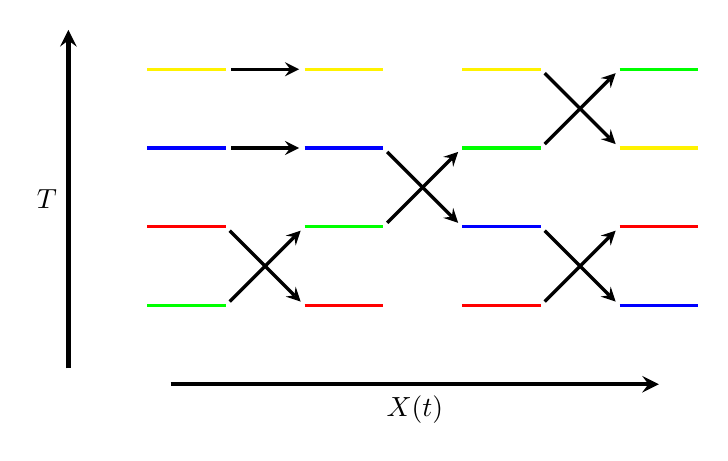
\begin{tikzpicture}
	    \draw[ultra thick,->,>=stealth] (1.3,0) -- (7.5,0) node[midway,below]{$X(t)$};
	    \draw[ultra thick,->,>=stealth] (0,0.2) -- (0,4.5) node[midway,left]{$T$};
	    
        \draw[very thick,green] (1,1) -- (2,1);
        \draw[very thick,red] (1,2) -- (2,2);
        \draw[very thick,blue] (1,3) -- (2,3);
        \draw[very thick,yellow] (1,4) -- (2,4);
        
        \draw[very thick,->,shorten >=2pt,shorten <=2pt,>=stealth] (2,1) -- (3,2);
        \draw[very thick,->,shorten >=2pt,shorten <=2pt,>=stealth] (2,2) -- (3,1);
        \draw[very thick,->,shorten >=2pt,shorten <=2pt,>=stealth] (2,3) -- (3,3);
        \draw[very thick,->,shorten >=2pt,shorten <=2pt,>=stealth] (2,4) -- (3,4);
        
        \draw[very thick,red] (3,1) -- (4,1);
        \draw[very thick,green] (3,2) -- (4,2);
        \draw[very thick,blue] (3,3) -- (4,3);
        \draw[very thick,yellow] (3,4) -- (4,4);
        
        \draw[very thick,->,shorten >=2pt,shorten <=2pt,>=stealth] (4,2) -- (5,3);
        \draw[very thick,->,shorten >=2pt,shorten <=2pt,>=stealth] (4,3) -- (5,2);
        
        \draw[very thick,red] (5,1) -- (6,1);
        \draw[very thick,blue] (5,2) -- (6,2);
        \draw[very thick,green] (5,3) -- (6,3);
        \draw[very thick,yellow] (5,4) -- (6,4);
        
        \draw[very thick,->,shorten >=2pt,shorten <=2pt,>=stealth] (6,1) -- (7,2);
        \draw[very thick,->,shorten >=2pt,shorten <=2pt,>=stealth] (6,2) -- (7,1);
        \draw[very thick,->,shorten >=2pt,shorten <=2pt,>=stealth] (6,3) -- (7,4);
        \draw[very thick,->,shorten >=2pt,shorten <=2pt,>=stealth] (6,4) -- (7,3);
        
        \draw[very thick,blue] (7,1) -- (8,1);
        \draw[very thick,red] (7,2) -- (8,2);
        \draw[very thick,yellow] (7,3) -- (8,3);
        \draw[very thick,green] (7,4) -- (8,4);        
	\end{tikzpicture}
	%	}
	\caption{A schematic representation of replica exchange molecular dynamics.}\label{Fig:ES:REMD}
\end{figure}

%\begin{figure}[htbp]
%    \centering
%	\includegraphics[width=0.6\textwidth]{figures/REMD.pdf}\\
%	\caption{A schematic representation of replica exchange molecular dynamics.}\label{Fig:ES:REMD}
%\end{figure}

Now, we exchange the temperatures of a pair of replicas
\begin{equation}
	\left\{ 
	\begin{array}{rcll} 
		x_m^{[i]}\equiv& \left(q^{[i]},p^{[i]}\right)_m \Rightarrow x_n^{[i]^\prime}&\equiv \left(q^{[i]},p^{[i]^\prime}\right)_n&\\ 
		&&&,\\
		x_n^{[j]}\equiv& \left(q^{[j]},p^{[j]}\right)_n \Rightarrow x_m^{[j]^\prime}&\equiv \left(q^{[j]},p^{[j]^\prime}\right)_m&\\  
	\end{array} 
	\right. 
\end{equation}
where
\begin{equation}
	\left\{ 
	\begin{array}{rl} 
		p^{[i]^\prime}\equiv \sqrt{\frac{T_n}{T_m}} p^{[i]}&\\ 
		&.\\
		p^{[j]^\prime}\equiv \sqrt{\frac{T_m}{T_n}} p^{[j]}&\\  
	\end{array} 
	\right. 
\end{equation}
The exchange rule is not trivial. In order for this exchange process to converge towards an equilibrium distribution, it is sufficient to impose the detailed balance condition on the transition probability $w(X\rightarrow X^\prime)$:
\begin{equation}
	W_{REM}(X)w(X\rightarrow X^\prime) = W_{REM}(X^\prime)w(X^\prime\rightarrow X).
\end{equation}
Then we have
\begin{align}
	&\frac{w\left(X\rightarrow X^\prime\right)}{w\left(X^\prime\rightarrow X\right)}\notag\\
	=&\frac{W_{REM}(X^\prime)}{W_{REM}(X)}\notag\\
	   =&\frac{\exp{\left(-\beta_m H\left(q^{[j]},p^{[j]^\prime}\right)\right)}\exp{\left(-\beta_n H\left(q^{[i]},p^{[i]^\prime}\right)\right)}}{\exp{\left(-\beta_m H\left(q^{[i]},p^{[i]^{ }}\right)\right)}\exp{\left(-\beta_n H\left(q^{[j]},p^{[j]^{ }}\right)\right)}}\notag\\
	   =&\frac{\exp{\left\{-\beta_m\left[K\left(p^{[j]^\prime}\right)+U\left(q^{[j]}\right)\right]-\beta_n\left[K\left(p^{[i]^\prime}\right)+U\left(q^{[i]}\right)\right]\notag\right\}}}
	   {\exp{\left\{-\beta_m\left[K\left(p^{[i]}\right)+U\left(q^{[i]}\right)\right]-\beta_n\left[K\left(p^{[j]}\right)+U\left(q^{[j]}\right)\right]\notag\right\}}}\notag\\
	   =&\frac{\exp{\left\{-\beta_m\left[\frac{T_m}{T_n}K\left(p^{[j]}\right)+U\left(q^{[j]}\right)\right]-\beta_n\left[\frac{T_n}{T_m}K\left(p^{[i]}\right)+U\left(q^{[i]}\right)\right]\notag\right\}}}
	   {\exp{\left\{-\beta_m\left[K\left(p^{[i]}\right)+U\left(q^{[i]}\right)\right]-\beta_n\left[K\left(p^{[j]}\right)+U\left(q^{[j]}\right)\right]\notag\right\}}}\notag\\
	   =&\dfrac{\exp{\left\{-\beta_n K\left(p^{[j]}\right)-\beta_m K\left(p^{[i]}\right)\right\}}}{\exp{\left\{-\beta_m K\left(p^{[i]}\right)-\beta_n K\left(p^{[j]}\right)\right\}}} \dfrac{\exp{\left\{-\beta_m U\left(q^{[j]}\right)-\beta_n U\left(q^{[i]}\right)\right\}}}{\exp{\left\{-\beta_m U\left(q^{[i]}\right)-\beta_n U\left(q^{[j]}\right)\right\}}}\notag\\
	   =&\exp{\left\{-\Delta\right\}}.
\end{align}
where $\Delta = \left[\beta_n-\beta_m\right]\left[U\left(q^{[i]}\right)-U\left(q^{[j]}\right)\right]$. It can be seen that the kinetic energy terms are fully canceled out.
This can be satisfied by the usual Metropolis criterion:
\begin{equation}
	w\left(X\rightarrow X^\prime\right)\equiv w\left(x_m^{[i]}\, \bigg\rvert\, x_n^{[j]}\right)= 
	\left\{ 
	\begin{array}{ll} 
		1, & \text{if } \Delta \leq 0\\ 
		\exp{(-\Delta)}, & \text{if } \Delta >0\\  
	\end{array} 
	\right. 
\end{equation}

The high-temperature replicas and the low-temperature replicas work in a collaborative way, in which the former explore phase space while the latter exploit phase space around local minima. The convergence rate is highly correlated to the acceptance ratio of exchange between neighboring replicas.  Kofke found that, for systems with Gaussian energy distributions, the average acceptance ratio is given by\cite{KofkeJCP2002,KofkeJCP2004a,KofkeJCP2004b}
\begin{equation}
	\left<\bar{p}_{acc}\right>=\erfc\left[\left(\frac{1}{2}C_v\right)^{1/2}\frac{1-\beta_j/\beta_i}{(1+(\beta_j/\beta_i)^2)^{1/2}}\right],
\end{equation}
where $C_v$ is the heat capacity at constant volume and is assumed to be constant in the temperature range between $\beta_i$ and $\beta_j$.
After long time simulations, all the replicas have arrived at a global equilibrium. In order to calculate the free energy or the ensemble average of an operator $\hat A$ at $T_m$, we can extract all the snapshots that have a temperature $T_m$ from $M$ trajectories, if this temperature was among the $M$ chosen temperatures. However, the optimal way is to use Weighted Histogram Analysis Method in Section~\ref{Sec:FEM:WHAM} or the Multistate Bennett Acceptance Ratio method in Section~\ref{Sec:FEM:MBAR}.  

In the above derivation, it only considers exchanges between neighboring states. However, a global permutation is also possible, and sometimes it may improve sampling efficiency.\cite{ChoderaJCP2011} REMD has been extended to Tsallis statistics\cite{WhitfieldPA2002}.

\subsection{Hamiltonian-Replica Exchange Molecular Dynamics\label{Sec:ES:REMD:HREMD}}
Another type of REMD simulation is called Hamiltonian replica exchange molecular dynamics (H-REMD), in which each replicas has its own Hamiltonian, but is coupled to the same temperature.\cite{JangPRL2003} One example is the H-REMD simulation for a torsional angle. The $m$th replica has a torsional energy term of 
\begin{equation}
	H_m(\phi)=\lambda(m)\sum_n\left(V_n/2\right)\left(1+\cos{\left[n\phi-\delta\right]}\right),
\end{equation}
where $\lambda$ is a control parameter. $\lambda(0)=1$ corresponds to the unbiased state and at $\lambda(M)$ (usually $\lambda(M)=0$) the torsional motion of this dihedral angle has a smaller barrier.

Another example of HREMD is pH-REMD, in which each replica is coupled with different pH of the solution. In other words, the chemical potential of hydronium in each replica is different . Therefore, the protonation states (or probability of being protonated or deprotonated) of titratable residues in each replica may differ from those in other replicas. In the simulations, the protonation states of titratable residues have their protonation states alternated according to the Metropolis criterion
\begin{equation}
	P= 
	\left\{ 
	\begin{array}{ll} 
		1, & \text{if } \Delta G_{\ce{P_{A}}\rightarrow \ce{P_{A}H^{+}}}\leq 0\\ 
		\exp{(-\beta\Delta G_{\ce{P_{A}}\rightarrow \ce{P_{A}H^{+}}})}, & \text{if }\Delta G_{\ce{P_{A}}\rightarrow \ce{P_{A}H^{+}}} >0\\  
	\end{array} 
	\right. 
\end{equation}
using Monte Carlo. The derivation of $\Delta G_{\ce{P_{A}}\rightarrow \ce{P_{A}H^{+}}}$ is shown below. 

Free energy of molecule \ce{A} in solution with a concentration $\left[\ce{A}\right]$
can be written as 
\[
\Delta G_{\ce{A}}=\Delta G_{\ce{A}}^{0}+\beta^{-1}\ln\frac{\left[\ce{A}\right]}{C_{0}},
\]
in which $\Delta G_{\ce{A}}^{0}$ is the free energy of molecule A at the standard
state $C_{0}$, i.e. 1 mol/L. The free energy change for a reaction
\begin{center}
	\schemestart \chemfig{A} + \chemfig{B} \arrow{<=>}[,0.75] \chemfig{C} \schemestop
\end{center}
%\[
%A+B\rightleftharpoons C
%\]
can be written as
\[
\Delta G=\Delta G_{\ce{C}}-\Delta G_{\ce{A}}-\Delta G_{\ce{B}}=\Delta G_{0}+\beta^{-1}\ln\frac{\left[\ce{C}\right]C_{0}}{\left[\ce{A}\right]\left[\ce{B}\right]}.
\]

At equilibrium, the free energy change is zero, we have
\begin{equation}
	\Delta G_{0}=-\beta^{-1}\ln\frac{\left[\ce{C}\right]C_{0}}{\left[\ce{A}\right]\left[\ce{B}\right]},\label{eq:FEM:REMD:standardfreeenergy}
\end{equation}
in which $\left[\ce{A}\right]\left[\ce{B}\right]/\left[\ce{C}\right]C_{0}$ is called
the dissociation constant $K_{a}$. So,

\begin{equation}
\Delta G_{0}=\beta^{-1}\ln K_{a}.
\label{eq:FEM:REMD:standardfreeenergyvsKa}
\end{equation}

Titration of a residue in a real protein can be written as
\begin{center}
	\schemestart \chemfig{P_{A}} + \chemfig{H^{+}} \arrow{<=>}[,0.75] \chemfig{P_{A}H^{+}} \schemestop
\end{center}
%\[
%P_{A}+H^{+}\rightleftharpoons P_{A}H^{+},
%\]

with 
\[
K_{a}=\frac{\left[\ce{P_{A}}\right]\left[\ce{H^{+}}\right]}{\left[\ce{P_{A}H^{+}}\right]C_{0}}
\]

The fraction of the deprotonated species is calculated as

\begin{eqnarray}
	f_{\left[\ce{P_{A}}\right]} & = & \frac{\left[\ce{P_{A}}\right]}{\left[\ce{P_{A}}\right]+\left[\ce{P_{A}H^{+}}\right]}\nonumber \\
	& = & \frac{1}{1+\frac{\left[\ce{P_{A}H^{+}}\right]}{\left[\ce{P_{A}}\right]}}\nonumber \\
	& = & \frac{1}{1+\frac{\left[\ce{P_{A}}\right]\left[\ce{H^{+}}\right]}{C_{0}K_{a}\left[\ce{P_{A}}\right]}}\nonumber \\
	& = & \frac{1}{1+\frac{1}{C_{0}K_{a}}\left[\ce{H^{+}}\right]}\nonumber \\
	& = & \frac{1}{1+\frac{1}{K_{a}}10^{-\mathrm{pH}}}\label{eq:FEM:REMD:titrationcurve}
\end{eqnarray}
We can check the asymptotic behavior of this equation. At strong
acidic condition ($\mathrm{pH}=-\infty$), $f_{\left[\ce{P_{A}}\right]}=0$, indicating that
the residue is 100 percent protonated. While at an extremely basic
condition ($\mathrm{pH}=\infty$), $f_{\left[\ce{P_{A}}\right]}=1$. This residue is 100
percent deprotonated. From the Henderson–Hasselbalch (HH) equation, 
the $\mathrm{p}K_a$ can be determined by the $\mathrm{pH}$ of the state when 
$\left[\ce{P_{A}}\right]/\left[\ce{P_{A}H^{+}}\right]=1$

\begin{align}
	\mathrm{p}K_{a}  = & -\log{K_{a}}\notag\\
	 = & -\log{\frac{\left[\ce{P_{A}}\right]}{\left[\ce{P_{A}H^{+}}\right]}}-\log{\frac{\left[\ce{H^{+}}\right]}{C_{0}}}\notag\\
	 = & -\log{\frac{\left[\ce{P_{A}}\right]}{\left[\ce{P_{A}H^{+}}\right]}}+\mathrm{pH}.
	 \label{eq:FEM:REMD:pKa}
\end{align}
The $\mathrm{p}K_{a}$ of each residue in a dipeptide has been determined by
experiment. However, when this residue is located in a certain protein,
its $\mathrm{p}K_{a}$ is different from that in the dipeptide. The difference
is called the $\mathrm{p}K_{a}$ shift. Instead of measuring the $\mathrm{p}K_{a}$
for a residue in a protein, we are more interested in calculating/measuring
the titration curve, which is the fraction of the deprotonated state
as a function of pH. From Eq.~\ref{eq:FEM:REMD:titrationcurve}, $f_{\left[P_{A}\right]}$
can be easily calculated if we know $K_{a}$ or equivalently the standard
free energy change of protonation in Eq.~\ref{eq:FEM:REMD:standardfreeenergyvsKa}.
The standard free energy can be calculated from the partition functions
as

\begin{eqnarray*}
	\Delta G_{0} & = & -\beta^{-1}\ln\frac{Q_{\ce{P_{A}H^{+}}}}{Q_{\ce{P_{A}}}Q_{\ce{H^{+}}}}\\
	& = & -\beta^{-1}\ln\frac{\iint\exp(-\beta E_{\ce{P_{A}H^{+}}})\diff \mathbf{R}_{H}\diff \mathbf{R}_{o}}{Q_{\ce{H^{+}}}\int\exp(-\beta E_{\ce{P_{A}}})\diff \mathbf{R}_{o}},
\end{eqnarray*}
where $\mathbf{R}_{H}$ is the coordinates of the specific \ce{H} atom and the other degrees-of-freedom (DoF) are denoted as $\mathbf{R}_{o}$. Generally, the absolute value of $\Delta G_{0}$ is hardly computable. A relative protonation free energy $\Delta\Delta G$ is preferred and is more reliable. Theoretically, the reference state can be any state you like. But the protonation free energy of the dipeptide is often used. The reference protonation process can be written as
\begin{center}
	\schemestart \chemfig{A} + \chemfig{H^{+}} \arrow{<=>}[,0.75] \chemfig{AH^{+}} \schemestop
\end{center}
%\[
%A+H^{+}\rightleftharpoons AH^{+}.
%\]

The free energy change from the reference state is 

\begin{align}
	&\Delta\Delta G_{0}\nonumber\\
	= & \Delta G_{0}-\Delta G_{0}^{ref}\nonumber \\
	= & -\beta^{-1}\ln\frac{\iint\exp(-\beta E_{\ce{P_{A}H^{+}}})\diff \mathbf{R}_{H}\diff \mathbf{R}_{o}}{Q_{\ce{H^{+}}}\int\exp(-\beta E_{\ce{P_{A}}})\diff \mathbf{R}_{o}}\frac{Q_{\ce{H^{+}}}\int\exp(-\beta E_{\ce{A}})\diff \mathbf{R}_{o}}{\iint\exp(-\beta E_{\ce{AH^{+}}})\diff \mathbf{R}_{H}\diff \mathbf{R}_{o}}\nonumber \\
	= & -\beta^{-1}\ln\frac{\iint\exp(-\beta E_{\ce{P_{A}H^{+}}})\diff \mathbf{R}_{H}\diff \mathbf{R}_{o}\int\exp(-\beta E_{\ce{A}})\diff \mathbf{R}_{o}}{\int\exp(-\beta E_{\ce{P_{A}}})\diff \mathbf{R}_{o}\iint\exp(-\beta E_{\ce{AH^{+}}})\diff \mathbf{R}_{H}\diff \mathbf{R}_{o}}\nonumber \\
	= & -\beta^{-1}\ln\frac{\iint\exp{\left[-\beta \left(E_{\ce{P_{A}H^{+}}}^{bond}+E_{\ce{P_{A}H^{+}}}^{QM}+E_{\ce{P_{A}H^{+}}}^{ele}\right)\right]}\diff \mathbf{R}_{H}\exp\left(-\beta E_{\ce{P_{A}H^{+}}}^{other}\right)\diff \mathbf{R}_{o}}{\iint\exp\left[-\beta \left(\ce{E_{AH^{+}}}^{bond}+E_{\ce{AH^{+}}}^{QM}+E_{\ce{AH^{+}}}^{ele}\right)\right]\diff \mathbf{R}_{H}\exp\left(-\beta E_{\ce{AH^{+}}}^{other}\right)\diff \mathbf{R}_{o}}\nonumber \\
	 & \cdot\frac{\int\exp\left(-\beta E_{\ce{A}}\right)\diff \mathbf{R}_{o}}{\int\exp\left(-\beta E_{\ce{P_{A}}}\right)\diff \mathbf{R}_{o}},\label{eq:FEM:REMD:Quotientofpartitionfunctions}
\end{align}
where $E^{bond}$
and $E^{ele}$ are the bonded energy and electrostatic interaction
energy related to this \ce{H} atom, respectively. $E^{QM}$ is the energy
correction that \textit{may} be required if the molecular mechanical
Hamiltonian cannot well capture the energy of the system, such as
the missing of charge transfer effect. The sum of the remaining energy
term is denoted as $E^{other}$, which does not explicitly depend
on the position of this specific \ce{H} atom. Eq.~\ref{eq:FEM:REMD:Quotientofpartitionfunctions}
is not ready to be computed before some approximations are adopted. 

\textit{First}, we assume that the total energy can be well described by the MM Hamiltonians
for both the state interested in and the reference state. Therefore,
\[
E_{\ce{P_{A}H^{+}}}^{QM}=E_{\ce{AH^{+}}}^{QM}=Const,
\]
and they can be removed from the integral. 

\textit{Second}, the bonded terms involving hydrogen atoms are usually 
constrained in the simulations. Therefore, the hydrogen atom in question has 
only one position and $E^{bond}=0$. Now, the 
relative protonation free energy can be simplified as
\begin{align}
\Delta\Delta G_{0}=&-\beta^{-1}\ln\frac{\int\exp\left(-\beta E_{\ce{P_{A}H^{+}}}^{ele}\right)\exp\left(-\beta E_{\ce{P_{A}H^{+}}}^{other}\right)\diff \mathbf{R}_{o}}{\int\exp\left(-\beta E_{\ce{AH^{+}}}^{ele}\right)\exp\left(-\beta E_{\ce{AH^{+}}}^{other}\right)\diff \mathbf{R}_{o}}\notag\\
&\cdot\frac{\int\exp\left(-\beta E_{\ce{A}}\right)\diff \mathbf{R}_{o}}{\int\exp\left(-\beta E_{P_{\ce{A}}}\right)\diff \mathbf{R}_{o}}.
\end{align}

Note that $E_{\ce{A}}=E_{\ce{AH^{+}}}^{other}$ and $E_{\ce{P_{A}}}=E_{\ce{P_{A}H^{+}}}^{other}$, we have
\begin{align}
	\Delta\Delta G_{0} = & -\beta^{-1}\ln\frac{\int\exp\left(-\beta E_{\ce{P_{A}H^{+}}}^{ele}\right)\exp\left(-\beta E_{\ce{P_{A}}}\right)\diff \mathbf{R}_{o}}{\int\exp\left(-\beta E_{\ce{P_{A}}}\right)\diff \mathbf{R}_{o}}\\
	& \cdot \frac{\int\exp\left(-\beta E_{\ce{A}}\right)\diff \mathbf{R}_{o}}{\int\exp\left(-\beta E_{\ce{AH^{+}}}^{ele}\right)\exp\left(-\beta E_{\ce{A}}\right)\diff \mathbf{R}_{o}}\\
	= & -\beta^{-1}\ln\left\langle \exp\left(-\beta E_{\ce{P_{A}H^{+}}}^{ele}\right)\right\rangle _{\ce{P_{A}}}\notag\\
	  &+\beta^{-1} \ln\left\langle \exp\left(-\beta E_{\ce{AH^{+}}}^{ele}\right)\right\rangle _{\ce{A}}\notag\\
	= & \Delta G_{\ce{P_{A}H^{+}}}^{ele}-\Delta G_{\ce{AH^{+}}}^{ele}  
\end{align}

Therefore,
\[
-\beta^{-1}\ln10\cdot \mathrm{p}K_{a}=\Delta G_{\ce{P_{A}H^{+}}}^{ele}-\Delta G_{\ce{AH^{+}}}^{ele}-\beta^{-1}\ln10\cdot \mathrm{p}K_{a}^{ref}.
\]

Using Eq.~\ref{eq:FEM:REMD:pKa}, at a certain pH the free energy difference between the deprotonated
and the protonated state can be written as

\[
\Delta G_{\ce{P_{A}}\rightarrow \ce{P_{A}H^{+}}}=\Delta G_{\ce{P_{A}H^{+}}}^{ele}+\beta^{-1}(\mathrm{pH}-\mathrm{p}K_{a}^{ref})\ln10-\Delta G_{\ce{AH^{+}}}^{ele}.
\]

In the above equation, $\Delta G_{\ce{AH^{+}}}^{ele}$ can be obtained from a free energy calculation of the model system by alchemically annihilation of the proton. However, $\Delta G_{\ce{P_{A}H^{+}}}^{ele}$ is unknown. Approximately, it can be replaced with $\Delta H_{\ce{P_{A}H^{+}}}^{ele}$ averaged over a few snapshots.\cite{MengJCTC2010} In order to accelerate the convergence,
this pH-REMD is often coupled with other enhanced simulation methods, such as T-REMD\cite{MengJCTC2010} and EDS-REMD\cite{LeeJCTC2014} (see section~\ref{Sec:ES:EDS}).
\clearpage
\input {chapters/SimulatedTempering.tex}
\clearpage
% !TeX spellcheck = en_US
% !TeX encoding = UTF-8
\section{Integrated Tempering Sampling\label{Sec:ES:ITS}}
Integrated tempering sampling (ITS) was proposed by Gao in 2008.\cite{GaoJCP2008}  It starts by writing a generalized distribution function $P(U)$, which is defined as the integration over $\beta$ in temperature space
\begin{equation}
	P(U)=\int f(\beta^\prime) e^{-\beta^\prime U}\diff \beta^\prime,
	\label{Eq:ES:ITS:distribution}
\end{equation}
where $f(\beta^\prime)$ is the weight, and if one takes $f(\beta^\prime)=\Omega(U)\delta(\beta - \beta^\prime)$ with $\Omega(U)$ being the density of states, the above equation returns to the unnormalized normal Boltzmann distribution function
\begin{equation}
	P(U)=\Omega(U)e^{-\beta U}.
\end{equation}
An energy function $U^\prime$ can be defined from this distribution function as
\begin{equation}
	U^\prime=-\beta^{-1}\ln \int f(\beta^\prime) e^{-\beta^\prime U}\diff \beta^\prime
\end{equation}
Correspondingly, the force can be calculated as
\begin{equation}
	\mathbf{F}^\prime=-\frac{\partial U^\prime}{\partial \mathbf{r}}=-\frac{\int \beta^{\prime} f\left(\beta^{\prime}\right) e^{-\beta^{\prime} U} d \beta^{\prime}}{\beta \int f\left(\beta^{\prime}\right) e^{-\beta^{\prime} U} d \beta^{\prime}} \frac{\partial U}{\partial \mathbf{r}}=\frac{\int \beta^{\prime} f\left(\beta^{\prime}\right) e^{-\beta^{\prime} U} d \beta^{\prime}}{\beta \int f\left(\beta^{\prime}\right) e^{-\beta^{\prime} U} d \beta^{\prime}} \mathbf{F} ,
\end{equation}
in which $\mathbf{F}$ is the force calculated from the original potential energy function of the system under study. A molecular dynamics simulation can be conducted using this force at the desired temperature $\beta$. The difficult part of this method is the determination of $f(\beta^\prime)$ that can yield an efficient sampling in the desired energy range.

Let $f(\beta^\prime)$ be a sum of delta functions
\begin{equation}
	f\left(\beta^{\prime}\right)=\sum_{k=1}^N n_k \delta\left(\beta^{\prime}-\beta_k\right) .
\end{equation}
With this, the distribution function in Eq.~\ref{Eq:ES:ITS:distribution} becomes
\begin{equation}
	P(U)=\sum_{k=1}^N n_k  e^{-\beta_k U}
\end{equation}
with weighting factors $n_k$ to be determined. By integration in  the entire configuration space, we find
\begin{equation}
	P_k= n_k \int e^{-\beta_k  U}\diff \mathbf{x}=\sum_{k=1}^N n_k Q_k,
\end{equation}
where $Q_k$ is the partition function at temperature $\beta_k$. One can preselect the ratios between $P_k$'s for all $k$'s between $1$ and $N$, and thus define a set of fixed expectation values $\{p_k^0\}$ for the normalized quantities $p_k$
\begin{equation}
	p_k=P_k/\sum_{k=1}^N P_k.
\end{equation}

However, the partition functions $Q_k$'s are unknown. Therefore, the desired distribution in terms of $\{p_k\}$ in an MD simulation can be achieved in an iterative procedure.
\begin{enumerate}
	\item Select a sequence of $\left\{\beta_k, k=1, N\right\}$ that cover the desired range of temperature.
	\item With a set of initial guess, $n_k(0)$, for $\left\{n_k, k=1, N\right\}$, a molecular dynamics simulation using force
	$$
	F_b=\frac{\sum_k \beta^{\prime} n_k e^{-\beta_k U}}{\beta \sum_k n_k e^{-\beta_k U}} F
	$$
	is conducted.
	\item $P_k$'s and thus $p_k$'s are calculated from the trajectory, and a new set of $\left\{n_k(1), k=1, N\right\}$ are obtained from $n_k(1)=n_k(0) p_k^0 / p_k$, followed by normalization.
	\item Repeat steps (2) and (3) to update $\left\{n_k, k=1, N\right\}$, until $\left\{p_k, k=1, N\right\}$ converges to $\left\{p_k^0, k=1, N\right\}$.
	\item Run MD simulations using the biased potential $U^\prime$ with the final set of $\left\{n_k, k=1, N\right\}$. The thermodynamic properties of the system are then calculated by reweighting of each term by multiplying a factor $e^{\beta\left(U^{\prime}(r)-U(r)\right)}=e^{-\beta U(r)} / P(U)$, with $P(U)$ being defined by Eq.~\ref{Eq:ES:ITS:distribution}.
\end{enumerate}

Introducing the idea of solute tempering into ITS leads to the selective integrated tempering sampling (SITS).\cite{YangJCP2009}
\clearpage
% !TeX spellcheck = en_US
% !TeX encoding = UTF-8
\section{Umbrella Sampling\label{Sec:ES:US}}
Umbrella Sampling method was proposed by Torrie and Valleau in 1977,\cite{TorrieJComputP1977} and is still widely used nowadays.
Suppose we are studying a transition process between two states such as conversion between two dominant conformations or a chemical reaction, and these two states are separated by a high barrier relative to $k_BT$. Therefore, the transition is a rare event. A schematic representation of the free energy landscape is shown in Fig.~\ref{Fig:ES:dual_harmonic}.
\begin{figure}[htbp]
	\centering
%	\resizebox{2cm}{!}{
		\begin{tikzpicture}
		\def\lims{xmin=-5,xmax=5.1,ymin=-38,ymax=14}
		\begin{axis}[\lims,hide x axis, hide y axis,width=0.65\textwidth,height=0.4\textwidth]
           \addplot[mark=none,smooth,domain=-5:5] {0.4*((x+2)*(x-2))*((x+2)*(x-2))-2*(x+0.5)*(x+0.5)-4};
           \draw[solid,->,>=Latex] (axis cs:-5,-29)--(axis cs:5,-29) node[below]{$\xi$};
		\end{axis}
		\end{tikzpicture}
%	}
	\caption{A typical free energy surface. Two free energy wells are separated by a barrier higher than $k_BT$.}\label{Fig:ES:dual_harmonic}
\end{figure}

%\begin{figure}[htbp]
%	\centering
%	\includegraphics[width=0.6\textwidth]{figures/dual_harmonic.pdf}\\
%	\caption{A typical free energy surface. Two free energy barriers are separated by a barrier higher than $kT$.}\label{Fig:ES:dual_harmonic}
%\end{figure}

Sometimes, we are interested in not only these two dominant states but also the whole pathway. Usually, we define a reaction coordinate $\xi$, including one or more collective variables (CVs), which can distinguish the two minima and characterize the free-energy pathway. Then we want to know the free-energy change along the reaction coordinate, $\xi$. It should be noted that choosing a suitable set of CVs is nontrivial for most cases.\cite{LeitoldJCP2020} A CV can be either a real coordinate such as the difference of bond lengths in, for example, an $S_N2$ reaction, or a thermodynamics coupling parameter ($\lambda$) that defines an unphysical path. If we run a simulation with the reaction coordinate set to a local maximum, i.e. the system being the transition state, the system will quickly roll back to the ``reactant'' or the ``product'' state in order to reduce the free energy. The consequence is that phase space outside the ``reactant'' and ``product'' regions cannot be sampled sufficiently to yield accurate free energy profile in a brute force simulation. In order to enhance the exploration in these regions, we can added a bias potential $\Delta V(\xi)$ into the system, guaranteeing
\begin{equation}
	\forall \xi_{1} \; \mathrm{and} \; \xi_{2}, \left [ U(\xi_{1}) + \Delta V(\xi_{1}) \right ]  - \left [ U(\xi_{2}) + \Delta V(\xi_{2}) \right ] < k_BT
\end{equation}
then the free-energy surface can be explored within the timescale amenable to MD simulations. $\Delta V(\xi)$ is called the ``umbrella potential''.

However, as the free-energy surface is usually not known \textit{a priori}, it is difficult to determine $\Delta V(\xi)$. To circumvent this issue, we can stratify the free-energy pathway into multiple \textit{windows}, namely break up the reaction-coordinate space into ``parts'', by a series of (usually harmonic) restraints, $\Delta U_i(\xi)$. In other words, the $i$th simulation, or the simulation of the $i$th window, is performed on the potential energy surface 
\begin{equation}
	U_i(\mathbf{R})=U_0(\mathbf{R})+\Delta U_i(\xi).
\end{equation}
The strengths of the biases should be strong enough to maintain the system in the vicinity of where you are interested in, and also should be weak enough that the system can have significant overlap between two adjacent windows. At the same time, the windows should be small enough to guarantee in each window,
\begin{equation}
	\forall \xi_{1} \; \mathrm{and} \; \xi_{2}, \left [ U(\xi_{1}) + \Delta U_i(\xi_{1}) \right ]  - \left [ U(\xi_{2}) + \Delta U_i(\xi_{2}) \right ] < k_BT
\end{equation}
After all the simulations, the (biased) distribution of the samples in the whole region should be as flat as possible. Ensemble average under $U_0$ can be calculated from the ensembles generated under the biased Hamiltonians $U$ via
\begin{align}
	\left<X(\mathbf{R})\right>_0=&\frac{\int X(\mathbf{R})\exp{\left[-\beta U_0(\mathbf{R})\right]}\diff\mathbf{R}}{\int \exp{\left[-\beta U_0(\mathbf{R})\right]}\diff\mathbf{R}}\notag\\
	                            =&\frac{\int X(\mathbf{R})\exp{\left[\beta \Delta U_i(\mathbf{R})\right]}\exp{\left[-\beta U_i(\mathbf{R})\right]}\diff\mathbf{R}}{\int \exp{\left[\beta \Delta U_i(\mathbf{R})\right]}\exp{\left[-\beta U_i(\mathbf{R})\right]}\diff\mathbf{R}}\notag\\
	                =&\frac{\left<X\exp{\left(\beta\Delta U_i\right)}\right>_i}{\left<\exp{\left(\beta\Delta U_i\right)}\right>_i}.
	\label{Eq:ES:US:reweighting}
\end{align}
Better postprocessing methods are the Weighted Histogram Analysis Method, Umbrella Integration and the Multistate Bennett Acceptance Ratio method (to be discussed in Section~\ref{Sec:FEM:WHAM}, ~\ref{Sec:FEM:UI} and~\ref{Sec:FEM:MBAR}).
\clearpage
% !TeX spellcheck = en_US
% !TeX encoding = UTF-8
\section{Accelerated Molecular Dynamics\label{Sec:ES:aMD}}
Accelerated molecular dynamics, or aMD for short, was proposed by Hamelberg et al in 2004,\cite{HamelbergJCP2004} based on the idea of hyperdynamics developed by Voter\cite{VoterPRL1997}.

In this method, the simulation is performed on the modified potential $V^\ast(\mathbf{r})$
\begin{equation}
	V^\ast(\mathbf{r})= 
	\left\{ 
	\begin{array}{rl} 
		V(\mathbf{r}), &\quad V(\mathbf{r})\geq E\\ 
		V(\mathbf{r})+\Delta V(\mathbf{r}), &\quad V(\mathbf{r})< E\\  
	\end{array} 
	\right.
\end{equation}
in which $E$ is a certain chosen energy, $\Delta V(\mathbf{r})$ is a continuous non-negative boost potential function, and $V(\mathbf{r})$ is the true potential. The bias potential increases the escape rate of the system from potential basins, and the subsequent state to state evolution of the system on the modified potential occurs at an accelerated rate with a nonlinear time scale of $\Delta t^\ast_i$, where
\begin{equation}
	\Delta t^\ast_i=\Delta t_i e^{\beta \Delta V(\mathbf{r}(t_i))}.
\end{equation}
The ensemble average value of any observable $A(\mathbf{r})$ taken on the modified potential can be written as
\begin{align}
	\left<A^\ast\right>=&\frac{\int \diff \mathbf{r}\,A(\mathbf{r})e^{-\beta V^{\ast}(\mathbf{r})}}{\int \diff \mathbf{r}\, e^{-\beta V^{\ast}(\mathbf{r})}}\notag\\
	        =&\frac{\int \diff \mathbf{r}\,A(\mathbf{r})e^{-\beta V(\mathbf{r})-\beta \Delta V(\mathbf{r})}}{\int \diff \mathbf{r}\, e^{-\beta V(\mathbf{r})-\beta \Delta V(\mathbf{r})}}.
\end{align}
The correct ensemble average can be written as
\begin{align}
	\left<A\right>=&\frac{\int \diff \mathbf{r}\,A(\mathbf{r})e^{-\beta V(\mathbf{r})}}{\int \diff \mathbf{r}\, e^{-\beta V(\mathbf{r})}}\notag\\
	=&\frac{\int \diff \mathbf{r}\,A(\mathbf{r})e^{-\beta V^\ast(\mathbf{r})+\beta \Delta V(\mathbf{r})}}{\int \diff \mathbf{r}\, e^{-\beta V^\ast(\mathbf{r})+\beta \Delta V(\mathbf{r})}}\notag\\
	=&\frac{\left<A(\mathbf{r})e^{\beta \Delta V(\mathbf{r})}\right>_{V^\ast}}{\left<e^{\beta \Delta V(\mathbf{r}) }\right>_{V^\ast}}.
\end{align}
Some technique can improve the numerical stability of this reweighting process.\cite{MiaoJCTC2014} The definition of $\Delta V(\mathbf{r})$ is non-unique, and Hamelberg et al proposed a modification of the potential energy surface more akin to snow drifts, which smooths the landscape by filling minima, but maintains the underlying shape of the unmodified potential energy surface and merges smoothly with the original potential at the threshold ``boost energy'' value $E$. It is defined as
\begin{equation}
	\Delta V(\mathbf{r})=\frac{(E-V(\mathbf{r}))^2}{\alpha+(E-V(\mathbf{r}))},
\end{equation}
where $\alpha$ is a tuning parameter that determines how deep the modified potential energy basin is (when $E-V(\mathbf{r})=\alpha, \Delta V(\mathbf{r})=\alpha/2$). With this biasing potential, the derivative of $V^{\ast}(\mathbf{r})$ has no discontinuity, and the modified potential reproduces the shape of the minima even at high value of $E$. Furthermore, $E$ should be carefully chosen, which may require a short trial simulation.

The most recent variant of aMD, the Gaussian accelerated molecular dynamics (GaMD), was developed by Miao et al\cite{MiaoJCTC2015}, in which the biasing potential is defined as
\begin{equation}
	\Delta V(\mathbf{r})= 
	\left\{ 
	\begin{array}{rl} 
		\frac{1}{2}k(E-V(\mathbf{r}))^2, &\quad V(\mathbf{r})< E\\ 
		0, &\quad V(\mathbf{r})\geq E\\  
	\end{array} 
	\right.
\end{equation}

In order to smoothen the potential energy surface for enhanced sampling, the boost potential needs to satisfy the following criteria. First, for any two arbitrary potential values $V(\mathbf{r}_1)$ and $V(\mathbf{r}_2)$ found on the original energy surface, $\Delta V$ should be a monotonic function that does no change the relative order of the biased potential values, i.e. 
\begin{equation}
	\sign{(V(\mathbf{r}_1)-V(\mathbf{r}_2))}=\sign{(V^\ast(\mathbf{r}_1)-V^\ast(\mathbf{r}_2))}.
\end{equation}
Without losing generality, let $V(\mathbf{r}_1)<V(\mathbf{r}_2)$, we have
\begin{equation}
	V^\ast(\mathbf{r}_1)<V^\ast(\mathbf{r}_2),
\end{equation}
which leads to
\begin{align}
    V(\mathbf{r}_1)+\frac{1}{2}k\left[E-V(\mathbf{r}_1)\right]^2-V(\mathbf{r}_2)-\frac{1}{2}k\left[E-V(\mathbf{r}_2)\right]^2<&0\notag\\
    \left[V(\mathbf{r}_1)-V(\mathbf{r}_2)\right]+\frac{1}{2}k\left[(2E-V(\mathbf{r}_1)-V(\mathbf{r}_2))(V(\mathbf{r}_2)-V(\mathbf{r}_1))\right]<&0\notag\\
    \left[V(\mathbf{r}_1)-V(\mathbf{r}_2)\right]\left[1-\frac{1}{2}k(2E-V(\mathbf{r}_1)-V(\mathbf{r}_2))\right]<&0.
\end{align}
Since $V(\mathbf{r}_1)<V(\mathbf{r}_2)$, we have
\begin{equation}
	1-\frac{1}{2}k(2E-V(\mathbf{r}_1)-V(\mathbf{r}_2))>0,
\end{equation}
or equivalently
\begin{equation}
	\text{Criterion 1: } E<\frac{1}{k}+\frac{1}{2}\left[V(\mathbf{r}_1)+V(\mathbf{r}_2)\right].
\end{equation}

Second, if $V(\mathbf{r}_1)<V(\mathbf{r}_2)$, the potential difference observed on the smoothened energy surface should be smaller than that of the original; i.e., $V^\ast(\mathbf{r}_2)-V^\ast(\mathbf{r}_1)<V(\mathbf{r}_2)-V(\mathbf{r}_1)$, which leads to
\begin{equation}
	\text{Criterion 2: } E>\frac{1}{2}\left[V(\mathbf{r}_1)+V(\mathbf{r}_2)\right].
\end{equation}
Therefore, the threshold energy must satisfy
\begin{equation}
	V_{\mathrm{max}}\leq E \leq V_{\mathrm{min}}+\frac{1}{k},
\end{equation}
where $V_{\mathrm{max}}$ and $V_{\mathrm{min}}$ are the maximum and minimum of potential energies, and $k$ has to satisfy
\begin{equation}
	k\leq \frac{1}{V_{\mathrm{max}}-V_{\mathrm{min}}}.
\end{equation}
It can be rewritten as
\begin{equation}
	k=k_0\frac{1}{V_{\mathrm{max}}-V_{\mathrm{min}}},
\end{equation}
where $k_0\in (0,1)$. $k_0$ determines the magnitude of the applied boost potential. With greater $k_0$, higher boost potential is added to the potential energy surface. The boost potential is
\begin{equation}
	\Delta V(\mathbf{r})=\frac{1}{2} k_{0} \frac{1}{V_{\max }-V_{\min }}(E-V(\mathbf{r}))^{2}, \quad V(\mathbf{r})<E.
\end{equation}

Third, the standard deviation of $\Delta V$ needs to be small enough (i.e., narrow distribution) to ensure accurate reweighting using cumulant expansion to the second order:\cite{MiaoJCTC2014}
\begin{equation}
	\sigma_{\Delta V}=\sqrt{\left(\left.\frac{\partial \Delta V}{\partial V}\right|_{V=V_{\mathrm{av}}}\right)^{2} \sigma_{V}^{2}}=k\left(E-V_{\mathrm{av}}\right) \sigma_{V} \leq \sigma_{0},
\end{equation}
where $V_{av}$ and $\sigma_{V}$ are the average and standard deviation of the system potential energies, and $\sigma_{\Delta V}$ is the standard deviation of $\Delta V$ with $\sigma_{0}$ as a user-specified upper limit (e.g., $10k_BT$) for accurate reweighting. If $E$ is set to the lower bound $E=V_{\mathrm{max}}$, we have
\begin{equation}
	k_{0} \leq \frac{\sigma_{0}}{\sigma_{V}} \frac{V_{\max }-V_{\min }}{V_{\max }-V_{\mathrm{av}}}.
\end{equation}
For efficient enhanced sampling with the highest possible acceleration, $k_0$ can then be set to its upper bound as
\begin{equation}
	k_{0}=\min \left(1.0, \frac{\sigma_{0}}{\sigma_{V}} \frac{V_{\max }-V_{\min }}{V_{\max }-V_{\mathrm{av}}}\right).
\end{equation}
Alternatively, when the threshold energy $E$ is set to its upper bound $E = V_{\mathrm{min}} + (1/k)$, we have
\begin{equation}
	k_{0} \geq\left(1-\frac{\sigma_{0}}{\sigma_{V}}\right) \frac{V_{\max }-V_{\min }}{V_{\mathrm{av}}-V_{\min }}.
\end{equation}
Then, we have
\begin{equation}
	\text{Criterion 3: } \left(1-\frac{\sigma_{0}}{\sigma_{V}}\right) \frac{V_{\max }-V_{\min }}{V_{\mathrm{av}}-V_{\min }} \leq k_0 \leq \frac{\sigma_{0}}{\sigma_{V}} \frac{V_{\max }-V_{\min }}{V_{\max }-V_{\mathrm{av}}}.
\end{equation}
\clearpage
\input {chapters/ABF.tex}
\clearpage 
% !TeX spellcheck = en_US
% !TeX encoding = UTF-8
\section{\texorpdfstring{$\lambda$-dynamics and extended-system dynamics}{λ-dynamics and extended-system dynamics}\label{Sec:ES:lambdadynamics}}
$\lambda$-dynamics was developed by Kong and Brooks in 1996.\cite{KongJCP1996} In this method, the coupling parameter $\lambda$ is treated as a pseudo particle with fictitious mass $m_\lambda$.
%\vspace{10pt}
The extended Hamiltonian for the system with a coupling parameter in one dimension can be written as
\begin{equation}
	H(\mathbf{R},\{\lambda_i, i=1,\dots,n\})=H_{Rxn}(\mathbf{R},\{\lambda_i\}) + \sum_{i=1}^n\frac{m_i}{2}{\dot{\lambda}_i}^2+U^{*}(\{\lambda_i\}),
\end{equation}
where $H_{Rxn}$ is a legitimate mapping provided that $H_{Rxn}(\mathbf{R},\lambda_i=0)$ and $H_{Rxn}(\mathbf{R},\lambda_i=1)$ correspond to the Hamiltonians for the reactant and product states respectively, and $U^{*}(\lambda)$ is a restraint that limits the range of $\lambda$. The pseudo particles can be coupled to high temperature baths, so it can have strengthened ability to overcome the barrier. However, this might lead to energy transfer between the pseudo degrees of freedom to the configuration degrees of freedom. Therefore, the fictitious mass $m_\lambda$ should be large enough to make this degree of freedom nearly adiabatic from the rest of the system.\cite{AbramsJCP2006} $\lambda$-dynamics can also be coupled with metadynamics,\cite{WuJPCL2011} which will be introduced in Sec.~\ref{Sec:ES:metadynamics}. For discussions on the robustness of this method, please refer to Ref.~\cite{BielerJCTC2014}.

In extended-system dynamics, which can be regarded as a ``geometric'' version of $\lambda$-dynamics, the extended Lagrangian is coupled with the usual Lagrangian. For the one-dimensional case,
\begin{equation}
	L(\mathbf{R})=L_{0}(\mathbf{R}) + \frac{m_\xi}{2}{\dot{\xi}}^2+U^{*}(\xi)
\end{equation}
Usually, pseudo springs are used to connect the extended and real CVs, namely
\begin{equation}
	U^{*}(\xi)=\frac{1}{2}k(\xi-\xi_{0}(\mathbf{R}))^{2}
\end{equation}
where $\xi_{0}(\mathbf{R})$ is the real CV, $\xi$ is the extended CV and $L_{0}(\mathbf{R})$ is the usual Lagrangian that drives the dynamics.

The method that makes the pseudo particles, namely $\xi$ in the one-dimensional case, coupled to high-temperature baths, is called temperature accelerated molecular dynamics (TAMD).\cite{MaraglianoCPL2006} 

In principle, extended-system dynamics can be coupled with many enhanced-sampling algorithms. In such cases, the biases are added on the pseudo particles instead of the real system. The combination of extended-system dynamics and ABF, called extended ABF (eABF)\cite{FuJCTC2016}, is practically useful, because i) ABF requires the second derivative of the collective variables to calculate the biasing forces, while in eABF, the biasing forces is directly obtained from the pseudo springs and ii) forces are vectors, implying in multidimensional case, biasing forces along different CVs may affect each other when they are not completely decoupled. While in eABF, the extended CVs are always independent.

For any extended-system-based enhanced-sampling algorithm, when the pseudo springs are hard enough, namely, $k$ is sufficiently large for each collective variable, there is approximately
\begin{equation}
	A(\xi_0)=A(\xi).
\end{equation}
This approximation is obvious if the spring is regarded as a two-force member. To estimate the free-energy profile rigorously, an umbrella-integration (UI)\cite{ZhengJCTC2012} or corrected $z$-averaged restraint (CZAR)\cite{LesageJPCB2017} estimator can be adopted. For the UI estimator, when the simulation reaches equilibrium, samples that satisfy
\begin{equation}
	\xi \in [\xi_{i}, \xi_{i+1})
\end{equation}
namely, $\xi$ of bin $i$ are extracted. Then these samples can be regarded as those from an umbrella sampling simulation, with the restraining center at $\frac{1}{2}(\xi_{i} + \xi_{i+1})$. Hence, the umbrella integration method can be used to estimate the free-energy profile,
\begin{equation}
	\frac{\partial A_{i}}{\partial \xi_{0}}=\frac{1}{\beta }\frac{\xi - \left \langle \xi_{0} \right \rangle_{\xi}}{(\sigma ( \xi_{0})_{\xi})^{2} }-k(\xi_{0} - \xi)
\end{equation}

For the CZAR estimator, the extended-system simulation is regarded as an adaptive umbrella-sampling one, and the umbrella potential comes from the spring. Hence,
\begin{equation}
	\frac{\partial A}{\partial \xi_0}=\frac{1}{\beta }\frac{\diff \ln p(\xi_0)}{\diff \xi_0} + k(\left \langle  \xi \right \rangle_{\xi_0}-\xi_0),
\end{equation}
where $p(\xi_0)$ is the observed distribution of $\xi_0$.

\clearpage 
\input {chapters/Wang_Landau.tex}
\clearpage 
\input {chapters/AWH.tex}
\clearpage
\input {chapters/metadynamics.tex}
\clearpage 
\input {chapters/VES.tex}
\clearpage 
% !TeX spellcheck = en_US
% !TeX encoding = UTF-8
\section{On-the-fly Probability Enhanced Sampling\label{Sec:ES:OPES}}
The On-the-fly Probability Enhanced Sampling (OPES) method was developed by Invernizzi and Parrinello in 2020.\cite{InvernizziJPCL2020} Different from the well-tempered metadynamics (WTMetaD), in which the biasing potential is defined independent of the probability distribution, the core idea of OPES is to update self-consistently the estimate of the probability distributions and of the biasing potential in an on-the-fly fashion. The probability distribution is constructed via reweighting and is used to estimate the biasing potential.

In order to converge to the flat distribution, the biasing potential at the $n^{th}$ step can be defined as
\begin{equation}
	V_n(\mathbf{s})=\frac{1}{\beta} \log{\hat{P}_n(\mathbf{s})},
\end{equation}
where $\hat{P}_n(\mathbf{s})$ is an estimate of the probability. However, in WTMetaD, we aim at reaching a target distribution $P^{tg}(\mathbf{s})$, which can be obtained if the bias is defined as
\begin{equation}
	V(\mathbf{s})=\frac{1}{\beta} \log{\frac{P(\mathbf{s})}{P^{tg}(\mathbf{s})}}.
\end{equation}
In WTMetaD,
\begin{equation}
	P^{tg}(\mathbf{s})\propto \left[P(\mathbf{s})\right]^{1/\gamma},
\end{equation}
which leads to
\begin{equation}
	V(\mathbf{s})=(1-1/\gamma)\frac{1}{\beta} \log{P(\mathbf{s})}.
\end{equation}

During the simulation, the estimated probability distribution is expressed as weighted sum of the Gaussian hills according to the previously deposited bias potential as
\begin{equation}
	\tilde{P}_n(\mathbf{s})=\frac{\sum_k^n w_k G(\mathbf{s},\mathbf{s}_k)}{\sum_k^n w_k},
\end{equation}
where the weights $w_k=e^{\beta V_{k-1}(\mathbf{s}_k)}$. The tilde above $P$ indicates that the probability distribution is not normalized. The normalization should be carried out with respect to the CV space, denoted as $\Omega_n$, actually explored up to step $n$. Thus, the normalization factor is
\begin{equation}
	Z_n=\frac{1}{|\Omega_n|}\int_{\Omega_n}\tilde{P}_n(\mathbf{s})\diff \mathbf{s}.
\end{equation}

With an additional positive term $\epsilon \ll 1$, the bias at the $n^{th}$ step becomes
\begin{equation}
	V(\mathbf{s})=(1-1/\gamma)\frac{1}{\beta} \log{\left(\frac{\tilde{P}_n(\mathbf{s})}{Z_n}+\epsilon\right)}.
\end{equation}
$\epsilon$ can also allow one to set a limit on the bias, thus providing better control over the desired exploration. It can be chosen to be $\epsilon=e^{-\beta \Delta E/(1-1/\gamma)}$, where $\Delta E$ is the height of the free energy barriers one wishes to overcome during the enhanced sampling. It leads to
\begin{equation}
	V(\mathbf{s})= -\Delta E
\end{equation}
without depositing biasing potential.
\clearpage 
\input {chapters/OSRW.tex}
\clearpage
\input {chapters/EDS.tex}
\clearpage
% !TeX spellcheck = en_US
% !TeX encoding = UTF-8
\section{Integrated Hamiltonian Sampling\label{Sec:ES:IHS}}
Integrated Hamiltonian sampling (IHS) was proposed by Cui in 2014.\cite{MoriJPCB2014} , motivated by the idea of Integrated Tempering Sampling.\ref{Sec:ES:ITS} In this method, the sampling is carried out using an effective Hamiltonian constructed by integrating the weighted Boltzmann distributions of a series of Hamiltonians. It also shares similar motivations as the enveloping distribution sampling (EDS) approach\ref{Sec:ES:EDS}.

With two ``end-state'' Hamiltonians with potential functions $U_0$ and $U_1$ and a series of intermediate Hamiltonians
\begin{equation}
	U_{\lambda}(\mathbf{R})=(1-\lambda)U_0(\mathbf{R})+\lambda U_1(\mathbf{R}),
\end{equation}
an effective Hamiltonian is defined as
\begin{equation}
	%U_b(\mathbf{R})=-\frac{1}{\beta} \ln \int_0^1 \mathrm{~d} \lambda \Omega(\lambda) \mathrm{e}^{-\beta U_\lambda(\mathbf{R})}
    U_b(\mathbf{R})=-\frac{1}{\beta} \ln \int_0^1 \mathrm{~d} \lambda \mathrm{e}^{-\beta \left[U_\lambda(\mathbf{R})-f_\lambda\right]}
\end{equation}
by integrating the distributions of the intermediate and end states. 
%Here, $\Omega(\lambda)$ is a weight function to be determined. 
Here, the contribution of each state to the integral is tuned by the shift $f_\lambda$ to the potential energy $U_\lambda(\mathbf{R})$. 
In practice, the integral above is discretized into a sum over
$N_{\lambda}$ windows
\begin{equation}
	%U_b(\mathbf{R})=-\frac{1}{\beta} \ln \sum_{i=1}^{N_\lambda} \Omega_i \mathrm{e}^{-\beta U_i(\mathbf{R})},
	U_b(\mathbf{R})=-\frac{1}{\beta} \ln \sum_{i=1}^{N_\lambda} \mathrm{e}^{-\beta \left[U_i(\mathbf{R})-f_i\right]},
\end{equation}
in which $U_i=U_{\lambda_i}$, 
%$\Omega_i=\Omega_{\lambda_i}$ 
$f_i=f_{\lambda_i}$
and $N_\lambda$ is the number of $\lambda$ grids. 

With the sampled configurational probability $\rho_b$, the unbiased and weighted probability distribution, $\rho_i$  and $\rho_i^{(b)}$, can be calculated via
\begin{equation}
	\frac{1}{Z_i} \rho_i(\mathbf{R})=\frac{1}{Z_b} \rho_b(\mathbf{R}) \mathrm{e}^{-\beta\left[U_i(\mathbf{R})-U_b(\mathbf{R})\right]},
\end{equation}
\begin{equation}
	\frac{1}{Z_i^{(b)}} \rho_i^{(b)}(\mathbf{R})=\frac{1}{Z_b} \rho_b(\mathbf{R}) \mathrm{e}^{-\beta\left[U_i(\mathbf{R})-f_i-U_b(\mathbf{R})\right]},
\end{equation}
where $Z_i=\int \rho_i(\mathbf{R})\diff \mathbf{R}$ and $Z_i^{(b)}=\int \rho_i^{b}(\mathbf{R})\diff \mathbf{R}$ are the configurational integrals. With this reweighting processing, any equilibrium thermodynamic properties of the end states can be computed from IHS straightforwardly.

The simplest way to optimize the contribution of each intermediate state to the integral is to set the expectation value of the probability for the weighted intermediate states to be uniform
\begin{equation}
	%-\beta^{-1} \ln \left\langle\Omega_i \mathrm{e}^{-\beta\left(U_i-U_b\right)}\right\rangle_b=-\beta^{-1} \ln \left\langle\Omega_j \mathrm{e}^{-\beta\left(U_j-U_b\right)}\right\rangle_b
	-\beta^{-1} \ln \left\langle \mathrm{e}^{-\beta\left(U_i-f_i-U_b\right)}\right\rangle_b=-\beta^{-1} \ln \left\langle\mathrm{e}^{-\beta\left(U_j-f_j-U_b\right)}\right\rangle_b,
\end{equation}
which leads to
\begin{equation}
	f_i-f_j=-\beta^{-1} \ln \frac{\left\langle\mathrm{e}^{-\beta\left(U_i-U_b\right)}\right\rangle_b}{\left\langle\mathrm{e}^{-\beta\left(U_j-U_b\right)}\right\rangle_b}
\end{equation}
or
\begin{equation}
	f_i=-\beta^{-1} \ln \left\langle\mathrm{e}^{-\beta\left(U_i-U_b\right)}\right\rangle_b+C_0=-\beta^{-1} \ln Z_i+C_0
\end{equation}
with $C_0$ being an arbitrary constant, which can be chosen such that $f_1=0$ or $\sum_i \exp(\beta f_i)=1$. It can be quickly realize that $f_i$ is the free energy of the unweighted state $i$.

However, $f_i$ is usually unknown before the simulation. In the histogram flattening approach, with an initial guess of $f_i^{(0)}$, it can be updated in an iterative fashion
\begin{equation}
	f_i^{(n+1)}=f_i^{(n)}+\Delta f_i^{(n)}
\end{equation}
with
\begin{equation}
	\begin{aligned}
		\Delta f_i^{(n)}= & -\beta^{-1} \ln \left\langle\mathrm{e}^{-\beta\left(U_i-f_i^{(n)}-U_b^{(n)}\right)}\right\rangle_b^{(n)} \\
		& -\min \left[\left\{-\beta^{-1} \ln \left\langle\mathrm{e}^{-\beta\left(U_j-f_j^{(n)}-U_b^{(n)}\right)}\right\rangle_b^{(n)}\right\}_j\right]
	\end{aligned}
\end{equation}
To avoid large oscillation and gently converge the shift $f_i$, a cap $\Delta f_{cap}$ can be applied on the amount to be updated per step:
\begin{equation}
	f_i^{(n+1)}=f_i^{(n)}+\min\left[\Delta f_i^{(n)},\Delta f_{cap}\right]
\end{equation}

To make a full use of all the configurations that have been sampled in the previous $n$ steps, WHAM can be a convenient yet powerful approach for the estimation of $f_i$
\begin{equation}
	\begin{aligned}
		f_i^{(n+1)}= & -\frac{1}{\beta} \ln \frac{\sum_{k=1}^n N^{(k)}\left\{\rho_i^{(b)}\right\}^{(k)}}{\sum_{l=1}^n N^{(l)} \exp \left[-\beta\left(f_i^{(l)}-g^{(l)}\right)\right]} \\
		& -\frac{1}{\beta} \ln C^{(n+1)}
	\end{aligned}
\end{equation}
and
\begin{equation}
	g^{(k)}=-\frac{1}{\beta} \ln \sum_{i=1}^{N_\lambda} \exp \left[-\beta\left(f_i^{(n+1)}+f_i^{(k)}\right)\right].
\end{equation}
\clearpage
%\input chapters/NEB.tex
%\clearpage
\input {chapters/string.tex}
\clearpage
\input {chapters/OAMS.tex}
